\pdfbookmark{Общая характеристика работы}{characteristic}             % Закладка pdf
\section*{Общая характеристика работы}

\newcommand{\actuality}{\pdfbookmark[1]{Актуальность}{actuality}\underline{\textbf{\actualityTXT}}}
\newcommand{\progress}{\pdfbookmark[1]{Разработанность темы}{progress}\underline{\textbf{\progressTXT}}}
\newcommand{\aim}{\pdfbookmark[1]{Цели}{aim}\underline{{\textbf\aimTXT}}}
\newcommand{\tasks}{\pdfbookmark[1]{Задачи}{tasks}\underline{\textbf{\tasksTXT}}}
\newcommand{\aimtasks}{\pdfbookmark[1]{Цели и задачи}{aimtasks}\aimtasksTXT}
\newcommand{\novelty}{\pdfbookmark[1]{Научная новизна}{novelty}\underline{\textbf{\noveltyTXT}}}
% \newcommand{\influence}{\pdfbookmark[1]{Практическая значимость}{influence}\underline{\textbf{\influenceTXT}}}
\newcommand{\methods}{\pdfbookmark[1]{Методология и методы исследования}{methods}\underline{\textbf{\methodsTXT}}}
\newcommand{\defpositions}{\pdfbookmark[1]{Положения, выносимые на защиту}{defpositions}\underline{\textbf{\defpositionsTXT}}}
\newcommand{\reliability}{\pdfbookmark[1]{Достоверность}{reliability}\underline{\textbf{\reliabilityTXT}}}
\newcommand{\probation}{\pdfbookmark[1]{Апробация}{probation}\underline{\textbf{\probationTXT}}}
\newcommand{\contribution}{\pdfbookmark[1]{Личный вклад}{contribution}\underline{\textbf{\contributionTXT}}}
\newcommand{\publications}{\pdfbookmark[1]{Публикации}{publications}\underline{\textbf{\publicationsTXT}}}
% \newcommand{\influenceTheoretical}{\textbf{\influenceTheoreticalTXT}}
% \newcommand{\influencePractiacal}{\textbf{\influencePracticalTXT}}
\newcommand{\influenceTheoretical}{\pdfbookmark[1]{Теоретическая значимость}{thereticalInfluence}\underline{\textbf{\influenceTheoreticalTXT}}}
\newcommand{\influencePractical}{\pdfbookmark[1]{Практическая значимость}{practicalInfluence}\underline{\textbf{\influencePracticalTXT}}}


{\actuality}

\ifsynopsis
%Этот абзац появляется только в~автореферате.

\else
%Этот абзац появляется только в~диссертации.

\fi

% {\progress}
% Этот раздел должен быть отдельным структурным элементом по
% ГОСТ, но он, как правило, включается в описание актуальности
% темы. Нужен он отдельным структурынм элемементом или нет ---
% смотрите другие диссертации вашего совета, скорее всего не нужен.

{\aim} 
диссертационной работы
разработка методики многокритериального сравнительного анализа алгоритмов дискретного
управления электропневматическим приводом на основе построения и
исследования фронтов Парето, обеспечивающей научно обоснованный выбор
оптимального алгоритма управления в соответствии с заданными эксплуатационными требованиями.

Предлагаемая методика основывается на многокритериальной оптимизации с использованием фронтов Парето
и суррогатных моделей, что позволяет обеспечить баланс между различными требованиями к качеству работы пневмопривода.

Для~достижения поставленной цели необходимо было решить следующие {\tasks}:
\begin{enumerate}[beginpenalty=10000] % https://tex.stackexchange.com/a/476052/104425
\item Разработать математические модели электропневматического привода с дискретными распределителями,
которые учитывают нелинейную динамику системы и дискретный характер управляющих воздействий для различных алгоритмов управления.

\item Проведение анализа существующих алгоритмов дискретного управления электропневматическим приводом и
методов их оптимизации для выявления основных характеристик и закономерностей функционирования системы

\item Разработка математических моделей и критериев оценки эффективности электропневматического привода с дискретными
распределителями, учитывающих как качество позиционирования, так и интенсивность переключений распределителей 
и остальных интересующих показателей качества.

\item Синтез и исследование различных алгоритмов дискретного управления электропневматическим приводом,
включая управление в скользящих режимах, ПИД-регулирование с ШИМ, нечеткое управление и прогнозное управление.

\item Разработка методов построения нейросетевых суррогатных моделей для аппроксимации зависимостей между
параметрами алгоритмов управления и показателями качества функционирования электропневматического привода.

\item Создание алгоритмов построения и анализа фронтов Парето для различных методов
управления с использованием суррогатных моделей и эволюционных алгоритмов оптимизации.

\item Разработка программно-аппаратного комплекса для
экспериментальных исследований электропневматического привода и верификации теоретических результатов.

\item Проведение сравнительного анализа эффективности различных алгоритмов управления на основе построенных фронтов Парето и
формирование рекомендаций по их практическому применению в зависимости от требований к системе.

Решение данных задач позволило создать комплексную методику многокритериального анализа и
обоснованного выбора алгоритмов управления электропневматическим приводом.
\end{enumerate}


{\novelty}
\begin{enumerate}[beginpenalty=10000] % https://tex.stackexchange.com/a/476052/104425
    \item Разработан новый подход к сравнительному анализу алгоритмов дискретного управления
    электропневматическим приводом, основанный на построении и исследовании фронтов Парето с
    использованием нейросетевых суррогатных моделей, что позволяет осуществлять научно
    обоснованный выбор алгоритма управления в соответствии с заданными требованиями к системе.

    \item Предложена модифицированная архитектура нейросетевой суррогатной модели на основе
    остаточных блоков для аппроксимации зависимостей между
    параметрами алгоритмов управления и показателями качества функционирования
    электропневматического привода, обеспечивающая повышенную точность
    прогнозирования и устойчивость к шуму в данных.

    \item Разработаны новые критерии оценки эффективности алгоритмов управления
    электропневматическим приводом, учитывающие как точность позиционирования, так
    и интенсивность переключений распределителей, что позволяет
    проводить комплексную оценку качества функционирования системы.

    \item Создан новый метод построения и анализа фронтов Парето для алгоритмов
    управления электропневматическим приводом, основанный на комбинации эволюционных
    алгоритмов оптимизации и суррогатного моделирования, что позволяет существенно сократить
    вычислительные затраты при сохранении точности результатов.

    \item Проведены экспериментальные исследования для верификации численных моделей и методик,
    что подтверждает их адекватность и применимость для реальных промышленных задач.
\end{enumerate}

{\influence} \ldots

{\methods} В рамках диссертационного исследования применялись теоретические и экспериментальные методы.
Теоретическая часть работы базируется на фундаментальных положениях теории автоматического 
управления, математического моделирования и оптимизации. При разработке математических моделей
электропневматического привода использовались методы термодинамики и механики сплошных
сред. Анализ динамики системы осуществлялся с применением методов качественной теории 
дифференциальных уравнений и теории устойчивости. Синтез алгоритмов управления проводился
с использованием теории скользящих режимов, нечеткой логики и прогнозного управления.

Для построения суррогатных моделей применялись методы глубокого обучения и нейросетевого
моделирования. Многокритериальная оптимизация параметров алгоритмов управления осуществлялась
с использованием эволюционных алгоритмов и теории Парето-оптимальности. Статистическая обработка
результатов выполнялась методами математической статистики и регрессионного анализа.

Экспериментальные исследования проводились на специально разработанном
лабораторном стенде с использованием современных средств измерения и
обработки данных. Верификация теоретических результатов осуществлялась
путем сравнительного анализа расчетных и экспериментальных данных.

Программная реализация алгоритмов управления и методов оптимизации
выполнена с использованием современных языков программирования Python и
Julia, а также специализированных библиотек для научных вычислений и машинного
обучения. Визуализация результатов осуществлялась с применением
современных графических средств и методов многомерного анализа данных.

Достоверность полученных результатов обеспечивается корректным применением
апробированных научных методов, согласованностью теоретических и экспериментальных
данных.

{\defpositions}
\begin{enumerate}[beginpenalty=10000] % https://tex.stackexchange.com/a/476052/104425

\item Методика многокритериального сравнительного анализа алгоритмов дискретного управления
электропневматическим приводом, основанная на построении и исследовании фронтов Парето
с использованием нейросетевых суррогатных моделей, обеспечивающая научно обоснованный
выбор оптимального алгоритма управления для заданных эксплуатационных требований.

\item Модифицированная архитектура нейронной сети с остаточными блоками для построения суррогатных моделей
электропневматического привода, позволяющая с высокой точностью
аппроксимировать зависимости между параметрами алгоритмов управления
и показателями качества функционирования системы при существенном сокращении вычислительных затрат.

\item Комплекс критериев оценки эффективности алгоритмов управления электропневматическим
приводом, учитывающий как точность позиционирования, так и интенсивность
переключений распределителей, позволяющий проводить всесторонний анализ качества
функционирования системы в различных режимах работы.

\item Метод построения и анализа фронтов Парето для алгоритмов управления электропневматическим
приводом на основе комбинации эволюционных алгоритмов оптимизации и суррогатного моделирования,
обеспечивающий существенное сокращение вычислительных затрат при сохранении точности результатов.

\item Результаты экспериментальных исследований, подтверждающие эффективность разработанной
методики многокритериального анализа и практические рекомендации по выбору алгоритмов
управления электропневматическим приводом в зависимости от требований к системе.

\end{enumerate}

{\reliability} 
полученных результатов обеспечивается применением строгого математического аппарата теории автоматического управления, 
методов оптимизации и численного моделирования; использованием апробированных методов термодинамики и механики для
построения математических моделей электропневматического привода; корректностью принятых допущений
при разработке математических моделей; применением современных методов машинного обучения и
статистического анализа при построении суррогатных моделей и обработке экспериментальных данных.

Теоретические положения и результаты моделирования подтверждаются данными экспериментальных
исследований, проведенных на специально разработанном лабораторном стенде с использованием
современных средств измерения и регистрации данных. Полученные результаты согласуются с известными
теоретическими положениями и экспериментальными данными других исследователей в области управления пневматическими системами.

Обоснованность научных положений и выводов подтверждается публикациями в рецензируемых
научных изданиях, положительной оценкой результатов работы на международных и всероссийских научных конференциях.

{\probation}
Основные результаты работы докладывались~на:
перечисление основных конференций, симпозиумов и~т.\:п.

{\contribution} 
Личный вклад автора заключается в разработке методики многокритериального
сравнительного анализа алгоритмов дискретного управления электропневматическим
приводом на основе построения и исследования фронтов Парето. Автором предложены
оригинальные модификации существующих алгоритмов управления, включая многорежимное
скользящее управление и нечеткое управление с расширенной базой правил, обеспечивающие улучшенные показатели качества позиционирования.

В рамках исследования автором разработана модифицированная архитектура
нейронной сети с остаточными блоками для построения суррогатных моделей электропневматического
привода. Предложен новый метод построения и анализа фронтов Парето на основе комбинации эволюционных
алгоритмов оптимизации и суррогатного моделирования. Сформулирован
комплекс критериев оценки эффективности алгоритмов управления,
учитывающий как точность позиционирования, так и интенсивность переключений распределителей.

Автором самостоятельно спроектирован и изготовлен экспериментальный
стенд, разработано программное обеспечение для проведения исследований,
выполнены все экспериментальные исследования и обработка их результатов
Проведена верификация теоретических результатов путем сравнения с экспериментальными
данными. На основе полученных результатов сформулированы практические рекомендации
по выбору алгоритмов управления электропневматическим приводом в зависимости от требований к системе.

Все основные результаты диссертационной работы получены автором самостоятельно.
Личный вклад в работах, опубликованных в соавторстве, заключается в
постановке задач исследования, разработке методов их решения, проведении
теоретических и экспериментальных исследований, анализе и обобщении полученных результатов.

\ifnumequal{\value{bibliosel}}{0}
{%%% Встроенная реализация с загрузкой файла через движок bibtex8. (При желании, внутри можно использовать обычные ссылки, наподобие `\cite{vakbib1,vakbib2}`).
    {\publications} Основные результаты по теме диссертации изложены
    в~XX~печатных изданиях,
    X из которых изданы в журналах, рекомендованных ВАК,
    X "--- в тезисах докладов.
}%
{%%% Реализация пакетом biblatex через движок biber
    \begin{refsection}[bl-author, bl-registered]
        % Это refsection=1.
        % Процитированные здесь работы:
        %  * подсчитываются, для автоматического составления фразы "Основные результаты ..."
        %  * попадают в авторскую библиографию, при usefootcite==0 и стиле `\insertbiblioauthor` или `\insertbiblioauthorgrouped`
        %  * нумеруются там в зависимости от порядка команд `\printbibliography` в этом разделе.
        %  * при использовании `\insertbiblioauthorgrouped`, порядок команд `\printbibliography` в нём должен быть тем же (см. biblio/biblatex.tex)
        %
        % Невидимый библиографический список для подсчёта количества публикаций:
        \phantom{\printbibliography[heading=nobibheading, section=1, env=countauthorvak,          keyword=biblioauthorvak]%
        \printbibliography[heading=nobibheading, section=1, env=countauthorwos,          keyword=biblioauthorwos]%
        \printbibliography[heading=nobibheading, section=1, env=countauthorscopus,       keyword=biblioauthorscopus]%
        \printbibliography[heading=nobibheading, section=1, env=countauthorconf,         keyword=biblioauthorconf]%
        \printbibliography[heading=nobibheading, section=1, env=countauthorother,        keyword=biblioauthorother]%
        \printbibliography[heading=nobibheading, section=1, env=countregistered,         keyword=biblioregistered]%
        \printbibliography[heading=nobibheading, section=1, env=countauthorpatent,       keyword=biblioauthorpatent]%
        \printbibliography[heading=nobibheading, section=1, env=countauthorprogram,      keyword=biblioauthorprogram]%
        \printbibliography[heading=nobibheading, section=1, env=countauthor,             keyword=biblioauthor]%
        \printbibliography[heading=nobibheading, section=1, env=countauthorvakscopuswos, filter=vakscopuswos]%
        \printbibliography[heading=nobibheading, section=1, env=countauthorscopuswos,    filter=scopuswos]}%
        %
        \nocite{*}%
        %
        {\publications} Основные результаты по теме диссертации изложены в~\arabic{citeauthor}~печатных изданиях,
        \arabic{citeauthorvak} из которых изданы в журналах, рекомендованных ВАК%
        \ifnum \value{citeauthorscopuswos}>0%
            , \arabic{citeauthorscopuswos} "--- в~периодических научных журналах, индексируемых Web of~Science и Scopus%
        \fi%
        \ifnum \value{citeauthorconf}>0%
            , \arabic{citeauthorconf} "--- в~тезисах докладов.
        \else%
            .
        \fi%
        \ifnum \value{citeregistered}=1%
            \ifnum \value{citeauthorpatent}=1%
                Зарегистрирован \arabic{citeauthorpatent} патент.
            \fi%
            \ifnum \value{citeauthorprogram}=1%
                Зарегистрирована \arabic{citeauthorprogram} программа для ЭВМ.
            \fi%
        \fi%
        \ifnum \value{citeregistered}>1%
            Зарегистрированы\ %
            \ifnum \value{citeauthorpatent}>0%
            \formbytotal{citeauthorpatent}{патент}{}{а}{}%
            \ifnum \value{citeauthorprogram}=0 . \else \ и~\fi%
            \fi%
            \ifnum \value{citeauthorprogram}>0%
            \formbytotal{citeauthorprogram}{программ}{а}{ы}{} для ЭВМ.
            \fi%
        \fi%
        % К публикациям, в которых излагаются основные научные результаты диссертации на соискание учёной
        % степени, в рецензируемых изданиях приравниваются патенты на изобретения, патенты (свидетельства) на
        % полезную модель, патенты на промышленный образец, патенты на селекционные достижения, свидетельства
        % на программу для электронных вычислительных машин, базу данных, топологию интегральных микросхем,
        % зарегистрированные в установленном порядке.(в ред. Постановления Правительства РФ от 21.04.2016 N 335)
    \end{refsection}%
    \begin{refsection}[bl-author, bl-registered]
        % Это refsection=2.
        % Процитированные здесь работы:
        %  * попадают в авторскую библиографию, при usefootcite==0 и стиле `\insertbiblioauthorimportant`.
        %  * ни на что не влияют в противном случае
        \nocite{vakbib2}%vak
        \nocite{patbib1}%patent
        \nocite{progbib1}%program
        \nocite{bib1}%other
        \nocite{confbib1}%conf
    \end{refsection}%
        %
        % Всё, что вне этих двух refsection, это refsection=0,
        %  * для диссертации - это нормальные ссылки, попадающие в обычную библиографию
        %  * для автореферата:
        %     * при usefootcite==0, ссылка корректно сработает только для источника из `external.bib`. Для своих работ --- напечатает "[0]" (и даже Warning не вылезет).
        %     * при usefootcite==1, ссылка сработает нормально. В авторской библиографии будут только процитированные в refsection=0 работы.
}
 % Характеристика работы по структуре во введении и в автореферате не отличается (ГОСТ Р 7.0.11, пункты 5.3.1 и 9.2.1), потому её загружаем из одного и того же внешнего файла, предварительно задав форму выделения некоторым параметрам

%Диссертационная работа была выполнена при поддержке грантов \dots

%\underline{\textbf{Объем и структура работы.}} Диссертация состоит из~введения,
%четырех глав, заключения и~приложения. Полный объем диссертации
%\textbf{ХХХ}~страниц текста с~\textbf{ХХ}~рисунками и~5~таблицами. Список
%литературы содержит \textbf{ХХX}~наименование.

\pdfbookmark{Содержание работы}{description}                          % Закладка pdf
\section*{Содержание работы}
Во \underline{\textbf{введении}} обосновывается актуальность
исследований, проводимых в~рамках данной диссертационной работы,
приводится обзор научной литературы по~изучаемой проблеме,
формулируется цель, ставятся задачи работы, излагается научная новизна
и практическая значимость представляемой работы.


\underline{\textbf{Первая глава}}
посвящена анализу современного
состояния позиционных пневмоприводов с дискретными распределителями.
Показано, что данный класс приводов представляет значительный интерес
благодаря низкой стоимости и высокой надежности, однако их эффективное
применение осложняется существенной нелинейностью динамических процессов,
обусловленной свойствами сжатого воздуха и дискретным характером управления.

Выявлены три противоречивых требования к характеристикам таких систем: обеспечение
высокой точности позиционирования, достижение требуемого быстродействия и минимизация
количества переключений распределителей. Установлено, что повышение точности
требует более частого переключения распределителей, что ускоряет износ аппаратуры,
а увеличение быстродействия негативно влияет на точность из-за возрастания динамических ошибок.

На основе анализа существующих исследований определено, что оптимальным
решением является структура с четырьмя дискретными распределителями, обеспечивающая
необходимую функциональность при сохранении простоты реализации. Показано,
что для эффективного решения задачи позиционирования необходим
интегративный подход к проектированию, учитывающий взаимосвязанность
процессов в пневматической, механической и управляющей подсистемах.

Сформулирована необходимость применения методов многокритериальной оптимизации,
в частности построения фронта Парето, для выявления предельно достижимых
характеристик привода. Определены основные направления исследований:
разработка уточненной математической модели пневмопривода;
синтез алгоритмов управления, обеспечивающих компромисс между
точностью позиционирования, быстродействием и интенсивностью
переключений распределителей; построение и анализ фронта
Парето для оптимизации параметров системы.

Во \underline{\textbf{второй главе}} разработана математическая модель
электропневматического привода с дискретными
распределителями. Представлена комплексная математическая модель, учитывающая механические,
термодинамические и пневматические процессы, а также особенности дискретного управления.

Исследуемый электропневматический привод представляет собой систему, состоящую из пневматического цилиндра
двустороннего действия с односторонним штоком, четырех дискретных двухпозиционных распределителей и
системы управления (рисунок \ref{fig:pneumatic_cylinder}). Ключевой особенностью рассматриваемой конфигурации
является использование двух
независимых распределителей для каждой полости цилиндра: один для подачи сжатого воздуха из магистрали,
другой для выхлопа в атмосферу.

\begin{figure}[ht]
	\centering
	\includegraphics[width=0.85\textwidth]{Dissertation/images/part2/расчетная_схема_привода.eps}
	\caption{Схема электропневматического привода с дискретными распределителями}
	\label{fig:pneumatic_cylinder}
\end{figure}

Получено уравнение механического движения поршня с учетом всех силовых факторов:
\begin{equation}
	M\ddot{x} = p_1F_1 - p_2F_2 - p_\text{атм}(F_1 - F_2) - R_\text{тр}(\dot{x}) - R_\text{упор}(x,\dot{x}).
\end{equation}

Для моделирования нелинейных эффектов трения применена модель LuGre:
\begin{equation}
	\frac{dz}{dt} = \dot{x} - \frac{\sigma_0|\dot{x}|}{g(\dot{x})}z,\quad
	R_\text{тр} = \sigma_0z + \sigma_1\dot{z} + \sigma_2v.
\end{equation}

На основе законов термодинамики получены уравнения для изменения давлений:
\begin{equation}
	\frac{dp_i}{dt} = \frac{\gamma}{V_i}\left(RT_i(G_{i\text{вх}} - G_{i\text{вых}}) \mp p_i F_i\frac{dx}{dt}\right).
\end{equation}

Массовый расход через распределители описан с помощью закона Сен-Венана-Ванцеля:
\begin{equation}
	G = \psi(p_1, p_2) \cdot C_d F_{max} \cdot u \frac{p_1}{\sqrt{RT_\text{вх}}},
\end{equation}
где $\psi(p_1, p_2)$ -- расходная функция, определяющая режим течения газа через распределитель.

Учтена динамика переключения распределителей: $\tau du/dt + u = u_{\text{зад}}$.
Полная математическая модель представлена системой из 9 дифференциальных уравнений,
решение которой осуществляется методом обратного дифференцирования (BDF) с адаптивным шагом.
С использованием разработанной модели исследованы динамические
характеристики пневмопривода. Выявлены и классифицированы 7
основных режимов функционирования из 16 теоретически возможных комбинаций состояний распределителей:

\begin{itemize}
	\item сильного положительного ускорения [1,0,0,1];
	\item умеренного положительного ускорения [1,0,0,0];
	\item слабого положительного ускорения [0,0,0,1];
	\item сильного отрицательного ускорения [0,1,1,0];
	\item умеренного отрицательного ускорения [0,0,1,0];
	\item слабого отрицательного ускорения [0,1,0,0];
	\item удержания [0,0,0,0];
\end{itemize}

Для каждого режима получены аналитические зависимости, характеризующие
динамику давлений и движение поршня. Установлено влияние
начальных условий на характер переходных процессов. Так, в режиме
умеренного положительного ускорения выявлено, что давление в штоковой полости
изменяется согласно зависимости $p_2V_2(x)^n = \text{const}$. Для режима удержания получено линеаризованное уравнение:
\begin{equation}
	M\ddot{x} + \left(\frac{\gamma p_{1,0}F_1^2}{V_{1,0}} + \frac{\gamma p_{2,0}F_2^2}{V_{2,0}}\right)x + \nu\dot{x} = 0.
\end{equation}

Построенные фазовые портреты и полученные математические зависимости позволяют
научно обоснованно подходить к выбору режимов работы при проектировании
алгоритмов управления пневмоприводом, обеспечивая требуемые показатели качества
позиционирования при минимизации количества переключений распределителей.


\underline{\textbf{Третья глава}}
посвящена разработке и исследованию методов управления позиционным
пневмоприводом с дискретными распределителями.

Разработан модифицированный ПИД-регулятор с ШИМ, включающий блок прогнозирования
тормозного пути. Математическая модель адаптивного торможения основана на анализе кинетической энергии системы:
\begin{equation}
	s_{\text{торм}}(t) = \frac{v(t)|v(t)|}{2a_{\text{торм}}} \cdot \left(1 + K_\text{нл} \cdot e^{-\frac{|v(t)|}{v_\text{хар}}}\right),
\end{equation}
где $v(t)$ -- скорость привода;
$a_{\text{торм}}$ -- желаемое ускорение торможения;
$K_\text{нл}$ -- коэффициент нелинейности;
$v_\text{хар}$ -- характерная скорость.

Результирующее управляющее воздействие формируется как комбинация сигналов:
\begin{equation}
	u_{\text{м}}(t) = (1 - k_{\text{торм}}(t))u_{\text{пид}}(t) + k_{\text{торм}}(t)u_{\text{торм}}(t),
\end{equation}
где интенсивность торможения $k_{\text{торм}}(t)$ определяется соотношением
между прогнозируемым тормозным путем и расстоянием до целевой точки.
Данная модификация устраняет перерегулирование при сохранении приемлемой
точности позиционирования. На алгоритм получено свидетельство о регистрации программы для ЭВМ.

\begin{figure}[h]
	\centering
	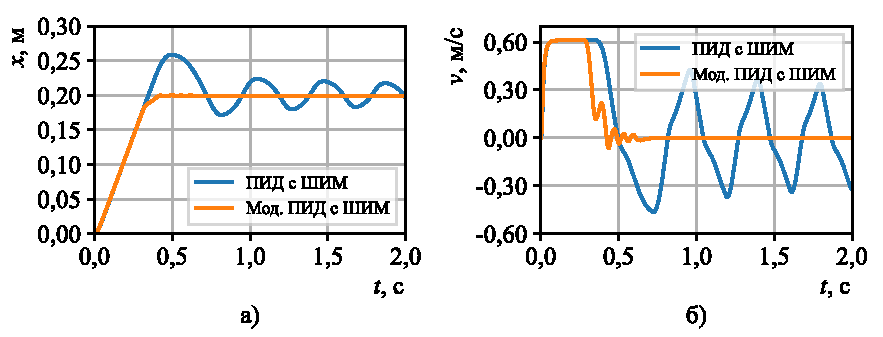
\includegraphics[width=\textwidth]{pid_comparison_2.pdf}
	\caption{Сравнение переходных процессов для классической и модифицированной структур ПИД-регулятора с ШИМ управлением}
\end{figure}

Для управления в скользящих режимах разработаны три конфигурации: трехрежимная, пятирежимная и семирежимная. Для пятирежимного управления закон имеет вид:
\begin{equation}
	\mathbf{u}(s) = \begin{cases}
		[1,0,0,1], & s > \varepsilon_2;                       \\
		[1,0,0,0], & \varepsilon_1 <   s \leq \varepsilon_2;  \\
		[0,0,0,0], & |s| \leq \varepsilon_1;                  \\
		[0,0,1,0], & -\varepsilon_2 <  s \leq -\varepsilon_1; \\
		[0,1,1,0], & s \leq -\varepsilon_2,
	\end{cases}
\end{equation}
где $s$ -- функция поверхности скольжения; $\varepsilon_1, \varepsilon_2$ -- параметры, определяющие границы зон переключения.

Исследованы две модификации поверхности скольжения: интегральная, обеспечивающая нулевую статическую ошибку:
\begin{equation}
	s_I = \dot{e} + \lambda_1 e + \lambda_2 \int_0^t e(\tau)d\tau,
\end{equation}
и терминальная, обеспечивающая конечное время сходимости:
\begin{equation}
	s_T = \dot{e} + \beta |e|^{q/p} \text{sign}(e),
\end{equation}
где $p$ и $q$ -- нечетные числа $(1 < q/p < 2)$; $\beta$ -- положительный коэффициент.

Установлено, что семирежимное управление обеспечивает наилучшее качество
позиционирования, создавая оптимальную градацию торможения.

Разработан нечеткий регулятор с двумя входными
лингвистическими переменными (ошибка позиционирования и скорость), характеризуемыми
пятью термами. База из 25 правил нечеткого вывода основывается на
знаниях физических процессов происходящих в рассматриваемом приводе.
Адаптивное изменение интенсивности
управляющего воздействия минимизирует число переключений распределителей.

Предложен оригинальный алгоритм прогнозного управления, основанный
на оптимизации на каждом шаге с использованием целевой функции:
\begin{equation}
	\begin{aligned}
		J & = \sum_{i=1}^{N_p} Q_{\text{поз}} \cdot (x(k+i|k) - x_{\text{зад}})^2 + \sum_{i=1}^{N_p} Q_{\text{скор}} \cdot v(k+i|k)^2 + \\
		  & + \sum_{i=0}^{N_c-1} R_{\text{перекл}} \cdot \sum_{j=1}^{4} |u_j(k+i|k) - u_j(k+i-1|k)|,
	\end{aligned}
\end{equation}
где $N_p$ -- горизонт прогноза; $N_c$ -- горизонт управления.

Для снижения вычислительных затрат разработан эвристический
алгоритм формирования пространства поиска, а так же упрощенная математическая модель позиционного пневмопривода.
Научно обоснованы оптимальные
значения горизонта прогноза $8 \leq N_p \leq 15$.

Проведенное исследование позволило определить преимущества и
ограничения каждого метода управления, что является основой для
выбора оптимальной структуры системы в зависимости от приоритетных требований.

\underline{\textbf{Четвертая глава}}
посвящена экспериментальной проверке разработанных математических моделей и алгоритмов
управления позиционным пневмоприводом с дискретными распределителями. Для проведения исследований
разработан специализированный лабораторный стенд, включающий пневмоцилиндр двустороннего действия с
односторонним штоком, четыре дискретных двухпозиционных распределителя, систему измерения и управления.

Экспериментальная установка реализована по иерархическому принципу и включает три основных уровня:
исполнительный уровень (датчики и актуаторы), уровень управления реального
времени (микроконтроллер STM32F767ZI) и уровень человеко-машинного
интерфейса (одноплатный компьютер Raspberry Pi 5). Система обеспечивает сбор данных с 24-битного
аналого-цифрового преобразователя с частотой дискретизации 1 кГц, реализацию
алгоритмов управления в реальном времени и визуализацию результатов через веб-интерфейс.

Программа экспериментального исследования включала следующие этапы:
\begin{enumerate}
	\item Экспериментальное определение параметров модели пневмопривода
	\item Получение и анализ экспериментальных данных о переходных процессах при различных алгоритмах управления
	\item Оценка адекватности разработанной математической модели
\end{enumerate}

Экспериментальное определение параметров модели включало тарировку потенциометрического
датчика положения Festo MLO-POT-450-TLF, измерение силы трения и времени срабатывания
распределителей. Тарировочная характеристика датчика описывается линейной зависимостью:
\begin{equation}
	x = \num{222.15}U - \num{16.00},
\end{equation}
где $x$ -- перемещение в миллиметрах, $U$ -- напряжение в вольтах.

Коэффициент детерминации $R^2 = \num{0.9998}$ подтверждает высокую линейность характеристики, а максимальная абсолютная погрешность не превышает \num{0.087} мм.
Для измерения силы трения проводились эксперименты в различных режимах: гармонические колебания,
постепенный разгон/торможение и многократные реверсы движения. Идентификация параметров модели трения
LuGre выполнялась методом наименьших квадратов с применением алгоритма Левенберга-Марквардта.
Полученные параметры
%(таблица \ref{tab1})
обеспечивают коэффициент детерминации $R^2 = \num{0.98229}$ при сравнении экспериментальной и модельной силы трения.
% \begin{table}[h]
% 	\centering
% 	\caption{Основные параметры модели трения LuGre}
% 	\label{tab1}
% 	\small
% 	\begin{tabular}{lll}
% 		\hline
% 		\textbf{Параметр} & \textbf{Значение} & \textbf{Единица измерения} \\
% 		\hline
% 		$f_c$             & \num{35.0718}     & Н                          \\
% 		$f_s$             & \num{47.1895}     & Н                          \\
% 		$v_s$             & \num{0.0151}      & \si{\metre\per\second}     \\
% 		$\sigma_0$        & \num{14280.0364}  & \si{\newton\per\metre}     \\
% 		\hline
% 	\end{tabular}
% \end{table}

Исследование времени срабатывания распределителей Camozzi A331-0C2 показало, что общее время
составляет примерно 31 мс как при открытии, так и при закрытии,
при этом стандартное квадратичное отклонение не превышает \num{2.1}~мс, что
свидетельствует о высокой повторяемости динамических характеристик.

Экспериментальное исследование переходных процессов позиционирования проводилось для четырех типов
алгоритмов управления: ПИД-регулятор с ШИМ, управление в скользящих режимах (УСР) с
различными конфигурациями, нечеткое управление и прогнозное управление. Для каждого алгоритма варьировались параметры настройки и регистрировались следующие показатели:

\begin{itemize}
	\item перемещение штока пневмоцилиндра $x(t)$;
	\item скорость движения $\dot{x}(t)$;
	\item давления в полостях пневмоцилиндра $p_1(t)$ и $p_2(t)$;
	\item комбинации состояний распределителей $\mathbf{u}(t)$;
	\item время переходного процесса $t_{\text{п}}$;
	\item статическая ошибка позиционирования $\Delta_{\text{ст}}$;
	\item перерегулирование $\sigma$;
	\item количество переключений между режимами $N_{\text{п}}$.
\end{itemize}

Сравнительный анализ экспериментальных данных (таблица \ref{tab2}) подтвердил
наличие компромисса между точностью позиционирования, быстродействием и ресурсными показателями системы.
\begin{table}[h]
	\centering
	\caption{Сравнительные характеристики алгоритмов управления}
	\label{tab2}
	\small
	\begin{tabular}{lccc}
		\hline
		\textbf{Алгоритм управления} & \textbf{Точность, мм} & \textbf{Время, с} & \textbf{Переключения} \\
		\hline
		ПИД с ШИМ                    & \num{0.60}            & \num{0.37}        & 272                   \\
		УСР-И-5                      & \num{0.62}            & \num{0.67}        & 17                    \\
		Нечеткая логика              & \num{0.95}            & \num{0.72}        & 9                     \\
		Прогнозное управление        & \num{0.80}            & \num{0.35}        & 7                     \\
		\hline
	\end{tabular}
\end{table}
ПИД-регулятор с ШИМ демонстрирует высокую частоту переключений распределителей
(272~--~527 за цикл), что негативно влияет на ресурс системы. Управление
в скользящих режимах с пятью градациями (УСР-И-5) обеспечивает хорошую точность
позиционирования (\num{0.62} мм) при значительно меньшем числе переключений (17). Нечеткое управление
характеризуется минимальным количеством переключений (9) при приемлемой точности (\num{0.95} мм).
Прогнозное управление демонстрирует оптимальное сочетание показателей: высокую точность (\num{0.80} мм),
минимальное время установления (\num{0.35} с) и наименьшее число переключений (7).
Оценка адекватности математической модели проводилась путем сравнения экспериментальных и
расчетных переходных процессов с использованием следующих метрик: коэффициент детерминации
$R^2$, среднеквадратичная ошибка $RMSE$ и относительная ошибка $\delta$. Для каждого алгоритма
управления оценивалось соответствие по четырем параметрам: перемещение штока, скорость,
давление в поршневой полости и давление в штоковой полости.

Результаты сравнительного анализа (рисцнок \ref{fig3}) показали, что разработанная математическая модель
с высокой точностью воспроизводит динамику пневмопривода для всех исследованных алгоритмов управления.
Наибольшую точность моделирования демонстрируют алгоритмы прогнозного управления (средняя относительная ошибка \num{4.36}\%)
и семирежимного управления в скользящих режимах с интегральной поверхностью (средняя ошибка \num{4.65}). Для алгоритмов
с высокой интенсивностью переключений, таких как ПИД-регулятор с ШИМ, относительная ошибка несколько выше (\num{5.87}\%).

\begin{figure}[h]
	\centering
	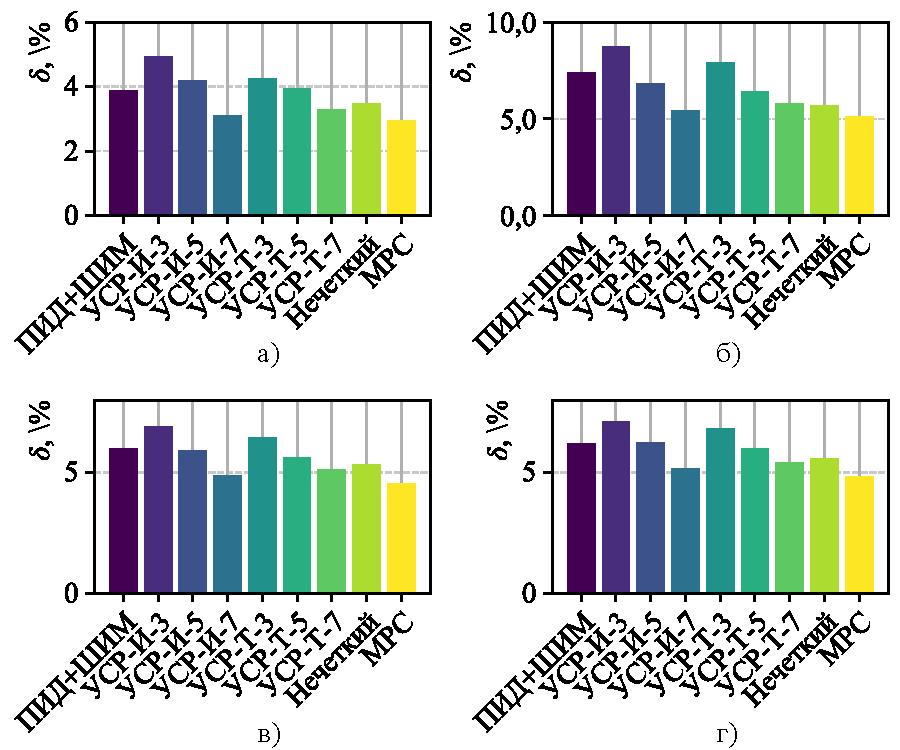
\includegraphics[width=0.9\textwidth]{Dissertation/images/part4/verification/delta_diagram.pdf}
	\caption{Сравнение точности моделирования различных алгоритмов управления по относительной ошибке $\delta$, \%\\
	а) перемещение штока; б) скорость движения; в) давление в поршневой полости; г) давление в штоковой полости}
	\label{fig3}
\end{figure}
Наиболее точно во всех случаях моделируется перемещение штока (среднее значение $R^2$ превышает \num{0.98}),
что важно для оценки точности позиционирования. Наибольшие расхождения наблюдаются при прогнозировании давлений
в полостях, что связано со сложностью моделирования термодинамических процессов.
Проведенные экспериментальные исследования подтвердили адекватность разработанной математической модели и
эффективность предложенных алгоритмов управления. Установлена высокая степень соответствия между результатами
математического моделирования и данными натурных экспериментов, что позволяет использовать разработанную методику
структурно-параметрического синтеза для оптимизации пневмоприводов с учетом требований по
точности позиционирования, быстродействию и ресурсу распределителей.

В \underline{\textbf{пятой главе}}
представлена методика многокритериального структурно-параметрического синтеза
позиционного пневмопривода с дискретными распределителями. Сформулирована задача структурно-параметрического
синтеза, включающая выбор оптимальной структуры управления и определение её параметров с учётом конфликтующих
требований к точности позиционирования, качеству переходных процессов и ресурсным показателям.

Для количественной оценки эффективности функционирования различных структур введены критерии
оптимизации: точность позиционирования ($AC$), интегральный критерий качества переходного процесса ($ITAE$) и
интенсивность переключений распределителей ($SI$), которые определяются следующими выражениями:
\begin{equation}
	AC = \lim_{t \to \infty} |e(t)| = \lim_{t \to \infty} |x_{\text{зад}} - x(t)|,
\end{equation}
\begin{equation}
	ITAE = \int_0^{T_{\text{мод}}} t |e(t)| dt,
\end{equation}
\begin{equation}
	SI = \sum_{i=1}^4 N_i,
\end{equation}
где $x_{\text{зад}}$ -- заданное положение,
$x(t)$ -- текущее положение штока,
$N_i$ -- количество переключений $i$-го распределителя.

Разработан алгоритм построения фронтов Парето, основанный на
применении замещающих суррогатных нейросетевых моделей с резидуальными блоками.
Показано, что использование метода латинского гиперкуба для формирования обучающей
выборки обеспечивает наиболее равномерное заполнение пространства параметров, что подтверждается оптимальным значением коэффициента Монте-Карло.

На основе построенных суррогатных моделей получены фронты Парето для девяти конкурсных
структур управления, включающих модифицированный ПИД-регулятор с ШИМ, управление в скользящих
режимах с различными поверхностями (интегральной и терминальной) и числом режимов (3, 5 и 7), нечёткое и прогнозное управление.

Для решения обратной задачи оптимизации разработан алгоритм поиска ближайшей
точки на фронте Парето к заданной целевой точке, основанный на нормализации критериев:
\begin{equation}
	\tilde{y}_i = \frac{y_i - y_{i,\min}}{y_{i,\max} - y_{i,\min}}, \quad i \in \{AC, ITAE, SI\},
\end{equation}
и применении взвешенной евклидовой нормы:
\begin{equation}
	\|\mathbf{\tilde{y}}(\mathbf{p}) - \mathbf{\tilde{y}}^*\|_w = \sqrt{\sum_{i} w_i (\tilde{y}_i(\mathbf{p}) - \tilde{y}_i^*)^2}.
\end{equation}

Предложенный метод коррекции параметров, базирующийся на
последовательных приближениях:
\begin{equation}
	\mathbf{p}^{(n+1)} = \mathbf{p}^{(n)} + \beta (\mathbf{y}^* - \mathbf{y}^{(n)}) \cdot \frac{\partial \mathbf{y}}{\partial \mathbf{p}}|_{\mathbf{p}^{(n)}},
\end{equation}
обеспечивает высокую точность нахождения оптимальных параметров управления.

В результате проведённого анализа фронтов Парето выделены предпочтительные
области применения различных структур управления и разработаны практические
рекомендации по их выбору. Установлено, что наивысшую точность позиционирования
(0,13~--~0,14 мм) обеспечивают семирежимное управление в скользящих режимах и прогнозное
управление, наилучшие динамические характеристики ($ITAE = \num{0,006}$ \si{\metre\per\second\square}) демонстрирует нечёткое управление, а наибольшее ресурсосбережение ($SI = 5$) -- пятирежимное управление в скользящих режимах с интегральной поверхностью.

Предложенная методика двухэтапного структурно-параметрического синтеза и сформированные
рекомендации обеспечивают возможность обоснованного выбора оптимальной
структуры пневмопривода с дискретными распределителями и определения её параметров для конкретных условий эксплуатации.


\FloatBarrier
\pdfbookmark{Заключение}{conclusion}                                  % Закладка pdf
В \underline{\textbf{заключении}} приведены основные результаты работы, которые заключаются в следующем:

\begin{enumerate}
	\item Разработана комплексная математическая модель позиционного пневмопривода с дискретными распределителями,
	      которая включает в себя как силовую, так и управляющую структуры. Модель учитывает нелинейные термодинамические
	      процессы в полостях пневмоцилиндра, переменную структуру системы при переключении распределителей, а также
	      динамические эффекты сухого и вязкого трения. Высокая степень согласованности результатов моделирования с
	      экспериментальными данными (расхождение не превышает 5~--~7\%) подтверждает адекватность и достоверность
	      разработанной модели для решения задач анализа и синтеза пневмоприводов различной структуры.

	\item Проведен комплексный анализ различных структур пневмопривода, что позволило выявить оптимальные
	      режимы переключения распределителей при позиционировании рабочего органа. Разработаны структуры управления
	      на основе различных принципов: модифицированная структура ПИД-регулятора с блоком прогнозирования тормозного пути,
	      управление в скользящих режимах с интегральной и терминальной поверхностями, нечеткое управление и прогнозное управление.
	      Экспериментальный анализ подтвердил, что прогнозное управление обеспечивает повышение точности позиционирования на 25~--~30\%
	      при одновременном сокращении числа переключений распределителей на 35~--~45\% по сравнению с традиционными алгоритмами.

	\item Проведен натурный эксперимент на специально разработанном лабораторном стенде, который подтвердил работоспособность
	      предложенных структур и высокую достоверность результатов, полученных с использованием разработанной математической модели.
	      Сравнительный анализ экспериментальных данных показал, что наибольшую точность моделирования демонстрируют алгоритмы прогнозного
	      управления и семирежимного управления в скользящих режимах, где средняя относительная ошибка не превышает 4,65\%.
	      Расхождение между расчетными и экспериментальными данными по основным показателям качества составляет
	      не более 7\% для всех исследованных алгоритмов управления.

	\item Разработана методика многокритериального структурно-\allowbreak па\-ра\-ме\-три\-че\-ско\-го синтеза, основанная
	      на использовании фронтов Парето с применением замещающей суррогатной нейросетевой модели. Для
	      формирования обучающей выборки применен метод латинского гиперкуба, обеспечивающий оптимальное
	      заполнение пространства параметров, что позволило сократить вычислительные затраты при построении
	      фронтов Парето на 48\%. Использование суррогатной модели обеспечило среднюю точность аппроксимации 91\%
	      при максимальном отклонении 12\%.

	\item Определена взаимосвязь между конфликтными статико-динамическими и ресурсными показателями
	      для позиционных пневмоприводов различной структуры на основе анализа фронтов Парето. Установлено,
	      что для ПИД-регулятора с ШИМ диапазон изменения критерия $ITAE$ составляет от 0,0298 до 0,0427 \si{\meter\per\second\square}
	      при изменении точности от 0,41 до 2,57 мм. Семирежимное управление с интегральной поверхностью
	      обеспечивает точность 0,13 мм при $ITAE = 0,019$ \si{\meter\per\second\square} и $SI = 15$, а прогнозное управление демонстрирует
	      точность 0,12 мм при $ITAE = 0,032$ \si{\meter\per\second\square} и $SI = 14$~--~$16$. Для нечеткого регулятора характерны
	      наилучшие показатели по критерию динамической эффективности ($ITAE = 0,006$ \si{\meter\per\second\square}) при точности 0,40 мм.

	\item Сформированы практические рекомендации по выбору оптимальной структуры позиционного
	      пневмопривода с дискретными распределителями. Выделены четыре предпочтительные области
	      применения различных алгоритмов управления:
	      \begin{itemize}
		      \item область высоконагруженных систем (УСР-И-5, MPC) с точностью 0,12~--~0,36 мм;
		      \item область точных манипуляторов (УСР-И-7) с точностью 0,14 мм;
		      \item область промышленной автоматики (УСР-Т-5, УСР-Т-7) с точностью 0,13~--~0,28 мм;
		      \item область простых систем (ПИД+ШИМ, УСР-И-3) с точностью 0,5~--~2,5 мм.
	      \end{itemize}
	      Определены рекомендуемые значения параметров алгоритмов управления для типовых задач
	      позиционирования, что позволяет сократить сроки проектирования и повышает эффективность разрабатываемых систем.
\end{enumerate}

Полученные результаты позволяют на научной основе выбирать оптимальную структуру и
параметры позиционного пневмопривода с дискретными распределителями в зависимости
от конкретных требований, существенно сокращая сроки проектирования и повышая
эффективность разрабатываемых систем.

% %% Согласно ГОСТ Р 7.0.11-2011:
%% 5.3.3 В заключении диссертации излагают итоги выполненного исследования, рекомендации, перспективы дальнейшей разработки темы.
%% 9.2.3 В заключении автореферата диссертации излагают итоги данного исследования, рекомендации и перспективы дальнейшей разработки темы.
В результате проведенного диссертационного исследования достигнута поставленная
цель комплексного повышения статико-динамических и ресурсных показателей позиционного пневмопривода с
дискретными распределителями в условиях их конфликтности. Получены следующие основные результаты:

\begin{enumerate}
    \item Разработана комплексная математическая модель позиционного пневмопривода с дискретными распределителями,
    которая включает в себя как силовую, так и управляющую структуры. Модель учитывает нелинейные термодинамические
    процессы в полостях пневмоцилиндра, переменную структуру системы при переключении распределителей, а также
    динамические эффекты сухого и вязкого трения. Высокая степень согласованности результатов моделирования с
    экспериментальными данными (расхождение не превышает 5~--~7\%) подтверждает адекватность и достоверность
    разработанной модели для решения задач анализа и синтеза пневмоприводов различной структуры.

    \item Проведен комплексный анализ различных структур пневмопривода, что позволило выявить оптимальные
    режимы переключения распределителей при позиционировании рабочего органа. Разработаны структуры управления
    на основе различных принципов: модифицированная структура ПИД-регулятора с блоком прогнозирования тормозного пути,
    управление в скользящих режимах с интегральной и терминальной поверхностями, нечеткое управление и прогнозное управление.
    Экспериментальный анализ подтвердил, что прогнозное управление обеспечивает повышение точности позиционирования на 25~--~30\%
    при одновременном сокращении числа переключений распределителей на 35~--~45\% по сравнению с традиционными алгоритмами.

    \item Проведен натурный эксперимент на специально разработанном лабораторном стенде, который подтвердил работоспособность
    предложенных структур и высокую достоверность результатов, полученных с использованием разработанной математической модели.
    Сравнительный анализ экспериментальных данных показал, что наибольшую точность моделирования демонстрируют алгоритмы прогнозного
    управления и семирежимного управления в скользящих режимах, где средняя относительная ошибка не превышает 4,65\%.
    Расхождение между расчетными и экспериментальными данными по основным показателям качества составляет
    не более 7\% для всех исследованных алгоритмов управления.

    \item Разработана методика многокритериального структурно-параметрического синтеза, основанная
    на использовании фронтов Парето с применением замещающей суррогатной нейросетевой модели. Для
    формирования обучающей выборки применен метод латинского гиперкуба, обеспечивающий оптимальное
    заполнение пространства параметров, что позволило сократить вычислительные затраты при построении
    фронтов Парето на 48\%. Использование суррогатной модели обеспечило среднюю точность аппроксимации 91\%
    при максимальном отклонении 12\%.

    \item Определена взаимосвязь между конфликтными статико-динамическими и ресурсными показателями
    для позиционных пневмоприводов различной структуры на основе анализа фронтов Парето. Установлено,
    что для ПИД-регулятора с ШИМ диапазон изменения критерия $ITAE$ составляет от 0,0298 до 0,0427 \si{\meter\per\second\square}
    при изменении точности от 0,41 до 2,57 мм. Семирежимное управление с интегральной поверхностью
    обеспечивает точность 0,13 мм при $ITAE = 0,019$ \si{\meter\per\second\square} и $SI = 15$, а прогнозное управление демонстрирует
    точность 0,12 мм при $ITAE = 0,032$ \si{\meter\per\second\square} и $SI = 14$~--~$16$. Для нечеткого регулятора характерны
    наилучшие показатели по критерию динамической эффективности ($ITAE = 0,006$ \si{\meter\per\second\square}) при точности 0,40 мм.

    \item Сформированы практические рекомендации по выбору оптимальной структуры позиционного
    пневмопривода с дискретными распределителями. Выделены четыре предпочтительные области
    применения различных алгоритмов управления:
    \begin{itemize}
        \item область высоконагруженных систем (УСР-И-5, MPC) с точностью 0,12~--~0,36 мм;
        \item область точных манипуляторов (УСР-И-7) с точностью 0,14 мм;
        \item область промышленной автоматики (УСР-Т-5, УСР-Т-7) с точностью 0,13~--~0,28 мм;
        \item область простых систем (ПИД+ШИМ, УСР-И-3) с точностью 0,5~--~2,5 мм.
    \end{itemize}
    Определены рекомендуемые значения параметров алгоритмов управления для типовых задач
    позиционирования, что позволяет сократить сроки проектирования и повышает эффективность разрабатываемых систем.
\end{enumerate}

Полученные результаты позволяют на научной основе выбирать оптимальную структуру и
параметры позиционного пневмопривода с дискретными распределителями в зависимости
от конкретных требований, существенно сокращая сроки проектирования и повышая
эффективность разрабатываемых систем.

\pdfbookmark{Литература}{bibliography}                                % Закладка pdf
% При использовании пакета \verb!biblatex! список публикаций автора по теме
% диссертации формируется в разделе <<\publications>>\ файла
% \verb!common/characteristic.tex!  при помощи команды \verb!\nocite!

\ifdefmacro{\microtypesetup}{\microtypesetup{protrusion=false}}{} % не рекомендуется применять пакет микротипографики к автоматически генерируемому списку литературы
\urlstyle{rm}                               % ссылки URL обычным шрифтом
\ifnumequal{\value{bibliosel}}{0}{% Встроенная реализация с загрузкой файла через движок bibtex8
	\renewcommand{\bibname}{\large \bibtitleauthor}
	\nocite{*}
	\insertbiblioauthor           % Подключаем Bib-базы
	%\insertbiblioexternal   % !!! bibtex не умеет работать с несколькими библиографиями !!!
}{% Реализация пакетом biblatex через движок biber
	% Цитирования.
	%  * Порядок перечисления определяет порядок в библиографии (только внутри подраздела, если `\insertbiblioauthorgrouped`).
	%  * Если не соблюдать порядок "как для \printbibliography", нумерация в `\insertbiblioauthor` будет кривой.
	%  * Если цитировать каждый источник отдельной командой --- найти некоторые ошибки будет проще.
	%
	%% authorvak
	\nocite{vakbib1}%
	\nocite{vakbib2}%
	\nocite{vakbib3}%
	\nocite{vakbib4}%
	\nocite{vakbib5}%
	\nocite{vakbib6}%
	\nocite{vakbib7}%
	\nocite{vakbib8}%
	\nocite{vakbib9}%
	\nocite{vakbib10}%
	\nocite{vakbib11}%
	\nocite{vakbib12}%
	\nocite{pub4}%
	\nocite{pub21}%
	\nocite{pub22}%
	%
	%% authorwos
	\nocite{wosbib1}%
	%
	%% authorscopus
	\nocite{scbib1}%
	%
	%% authorpatent
	\nocite{patbib1}%
	%
	%% authorprogram
	\nocite{progbib1}%
	%
	%% authorconf
	\nocite{pub3}
	\nocite{pub8}
	\nocite{pub13}
	\nocite{pub14}
	\nocite{pub16}
	\nocite{pub19}
	\nocite{pub20}
	%
	%% authorother
	\nocite{pub6}%


	\ifnumgreater{\value{usefootcite}}{0}{
		\begin{refcontext}[labelprefix={}]
			\ifnum \value{bibgrouped}>0
				\insertbiblioauthorgrouped    % Вывод всех работ автора, сгруппированных по источникам
			\else
				\insertbiblioauthor      % Вывод всех работ автора
			\fi
		\end{refcontext}
	}{
		\ifnum \totvalue{citeexternal}>0
			\begin{refcontext}[labelprefix=A]
				\ifnum \value{bibgrouped}>0
					\insertbiblioauthorgrouped    % Вывод всех работ автора, сгруппированных по источникам
				\else
					\insertbiblioauthor      % Вывод всех работ автора
				\fi
			\end{refcontext}
		\else
			\ifnum \value{bibgrouped}>0
				\insertbiblioauthorgrouped    % Вывод всех работ автора, сгруппированных по источникам
			\else
				\insertbiblioauthor      % Вывод всех работ автора
			\fi
		\fi
		%  \insertbiblioauthorimportant  % Вывод наиболее значимых работ автора (определяется в файле characteristic во второй section)
		\begin{refcontext}[labelprefix={}]
			\insertbiblioexternal            % Вывод списка литературы, на которую ссылались в тексте автореферата
		\end{refcontext}
		% Невидимый библиографический список для подсчёта количества внешних публикаций
		% Используется, чтобы убрать приставку "А" у работ автора, если в автореферате нет
		% цитирований внешних источников.
		\printbibliography[heading=nobibheading, section=0, env=countexternal, keyword=biblioexternal, resetnumbers=true]%
	}
}
\ifdefmacro{\microtypesetup}{\microtypesetup{protrusion=true}}{}
\urlstyle{tt}                               % возвращаем установки шрифта ссылок URL
